\documentclass[12pt,a4paper]{article}

\usepackage[german]{babel}
\usepackage[utf8]{inputenc}
\usepackage[pdftex]{graphicx}
\usepackage{fancyhdr,lastpage}
\usepackage{enumerate}
\usepackage{amsmath, amsthm, amssymb}
\usepackage[top=3cm, bottom=3cm, left=2cm, right=2cm]{geometry}
\usepackage{minitoc}
\usepackage{multicol}
\pagestyle{fancy}

% Header
\lhead{Projekt Almond}
\chead{Abschlussbericht}
\rhead{Seite \thepage /\pageref{LastPage} }

\begin{document}

\begin{titlepage}
	\begin{center}
		
\includegraphics[height=15cm]{./logo.pdf}\\
		{\LARGE \bf Abschlussbericht}\\[0.3cm]
	\end{center}
\end{titlepage}

\tableofcontents

\newpage

% Inhalt

\section{Übersicht}
Almond ({\bf A}utonomous {\bf L}ogging and {\bf M}anagement of {\bf N}etworked {\bf D}evices) ist ein System aus vernetzten Aktoren und Sensoren: Nuts ({\bf N}etworked {\bf Ut}ilities and {\bf S}ensors), die über einen zentralen Controller (Squirrel) gesteuert werden. Zusätzlich gibt es ein Backend für PCs, welches über eine Weboberfläche Zugriff auf Gerätedaten gibt und die Steuerung der Aktoren sowie Konfigurationsänderungen erlaubt.\\
Die einzelnen Geräte werden über ein dafür entwickeltes Protokoll via Bluetooth mit dem Controller verbunden. Der Controller selbst wird dann ebenfalls über Bluetooth mit dem auf einem Linux/Windows/Mac laufenden Backend verbunden. Dabei werden auch Logdaten (Verlauf der Sensor-Werte) mit übermittelt, die dann später auf dem Rechner ausgewertet werden können.

\section{Protokolle}
Um die Kommunikation zwischen den Nuts und dem Squirrel, sowie des Squirrels zum Backend zu gewährleisten sind zwei Protokolle entworfen worden.\\
Die Protokollpakete sind folgendermaßen aufgebaut:
\\
\\
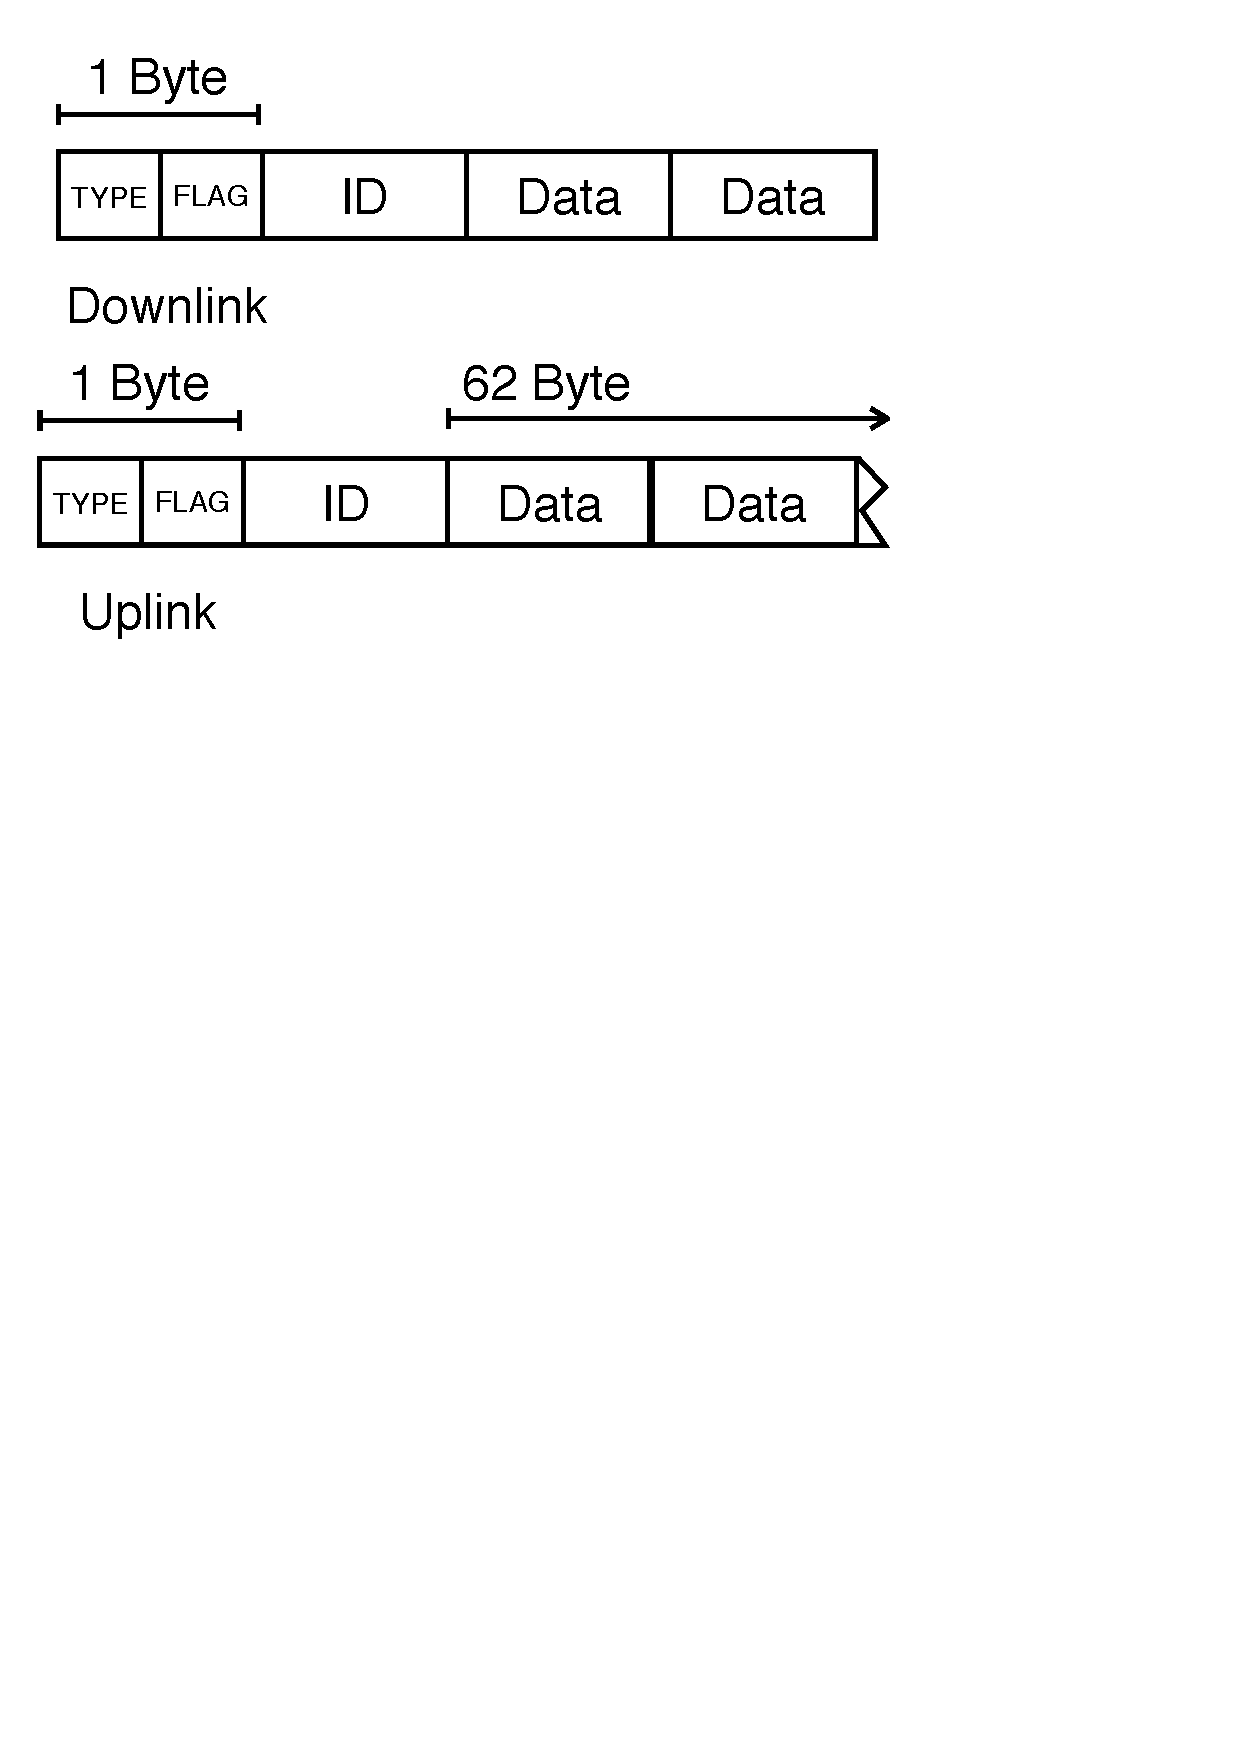
\includegraphics[height=6.5cm]{./ProkollDiagrams.pdf}\\

	\subsection{Downlink}  
Das Downlinkprotokoll dient zur Kommunikation der Nuts mit dem Squirrel.\\
Im Protokoll sind folgende enhalten: SET, GET, ECHO, BYE\\
Durch die Reduzierung auf diese geringe Anzahl an Befehlen, wird eine sehr kleine Paketgröße von 4 Bytes erreicht.\\
Neben dem Opcode findet sich in einem Paket eine ID mit der Aktoren oder Sensoren angesprochen werden können. Sowie ein 16 Bit-Wert, der für Nutzdaten verwendet werden kann.\\
\begin{itemize}
	\item{SET}
Der SET-Befehl kann Aktoren auf bestimmte Werste setzen.
	\item{GET}
Der GET-Befehl liest die akutellen Sensorewerte oder den Zustand eines Aktors aus.
	\item{ECHO}
Der ECHO-Befehl dient Debugging-Zwecken und sendet das empfangene Paket unverändert zurück.
	\item{BYE}
Der BYE-Befehl zeigt das Ende einer Verbindung an.
\end{itemize}
Um Variationen des GET-Befehls zu ermöglichen, wurden zusätzlich noch Flags implementiert.\\
\begin{itemize}
	\item{STANDARD}
Dieses Flag für die beeinflusst die Ausführung des Befehls nicht.
	\item{INFO\_NUT}
Dieses Flag dient dazu allgemeine - Sensor und Aktor unspezifische - Informationen der Nut, wie z.B. deren Namen abzurufen. Das übergebene ID-Feld wird nicht berücksichtigt.\\
	\item{INFO\_EXTENSION}
Mit diesem Flag werden Metdaten über den ausgewählten Sensor oder Aktor abgerufen.
\end{itemize}

	\subsection{Uplink}
Das Uplinkprotokoll dient zur Kommunikation zwischen dem Squirrel und dem Backend.\\
Zum einen wird mit diesem Protokoll das Squirrel durch das Backend konfiguriert. Zum anderen kann das Backend Informationen über die aktuell verfügabren Sensoren und Aktoren sowie deren Logdaten abrufen.\\
Es existieren folgende Befehle:
\begin{itemize}
	\item{LIST}
Teilt dem Backend alle verfügbaren Meta-Daten der Nuts, wie z.B. deren Bluetooth-Adresse, deren Sensoren und Aktoren, mit. Die Mess- und Zustandswerte selbst werden nicht übertragen.

	\item{LOG}
Mit diesem Befehle werden die in der Squirrel zwischengespeicherten Sensorwerte der verschiedenen Nuts dem Backend mitgeteilt.

	\item{TIME}
Mit diesem Befehl, kann das Backend die aktuelle Zeit der Squirrel mitteilen.

\end{itemize}
Hier ein schematischer Kommunikationsablauf zwischen Backend, Squirrel und Nut:\\ 
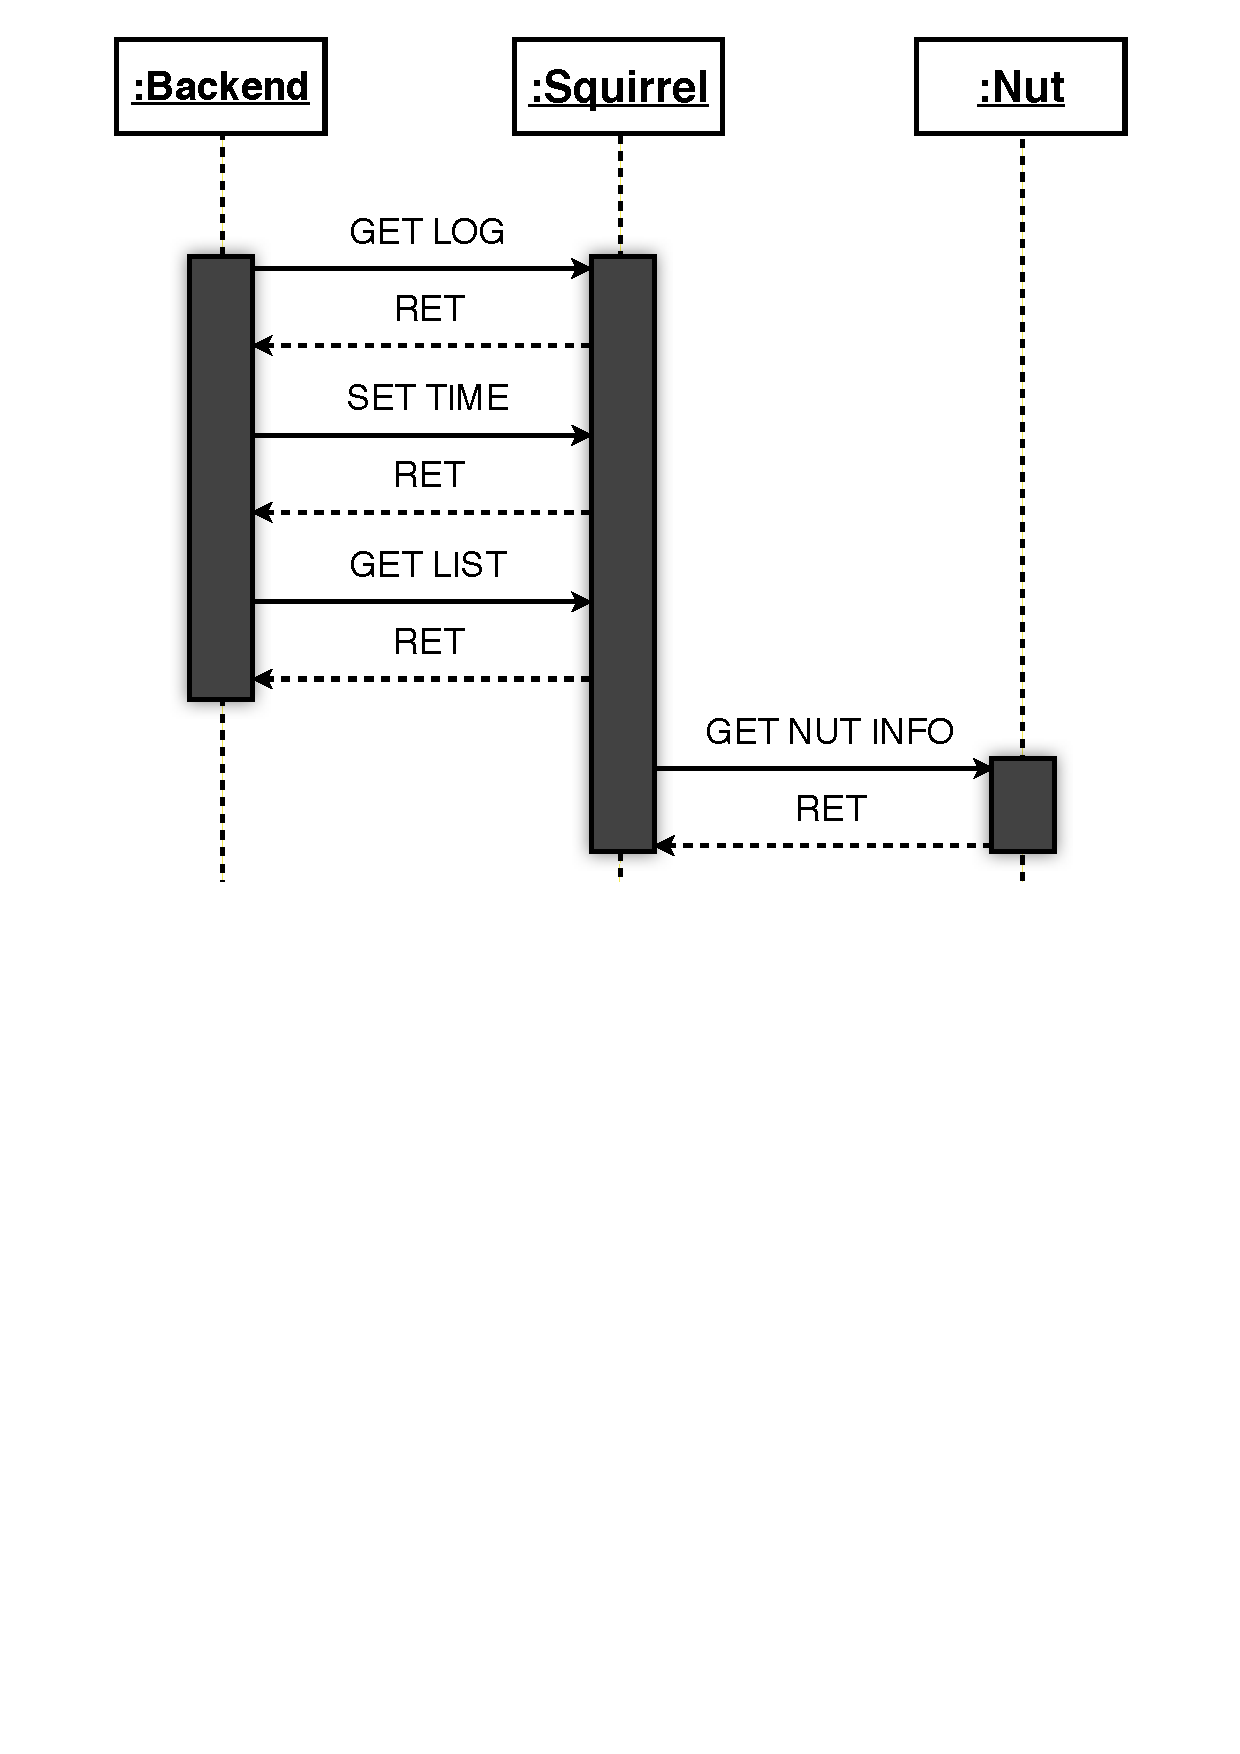
\includegraphics[height=8cm]{./ProtokollSequence.pdf}\\

\section{Interfaces}
Die im folgenden beschriebenen Interfaces sind die Schnittstellen um die im Almond-Projekt vorhandenen Sensoren und Aktoren direkt auf Hardwareebene ansprechen zu können.
	\subsection{UART}
Universal Asynchronous Receiver/Transmitter wird im Almond-Projekt für die Anbindung der Bluetoothmodule sowohl auf der Nut als auch der Squirrel verwendet.


	\subsection{SPI}
Das Serial Perpheral Interface verfügt über 4 Pins, welche mit Master-Out-Slave-In (MOSI), Master-In-Slave-Out (MISO), CLOCK und Slave-Select (SS).
\begin{itemize}
\item MOSI
Der MOSI Pin stellt die Datenleitung vom Master zum Slave dar.
\item MISO
Der MISO Pin stellt die Datenleitung vom Slave zum Master dar.
\item CLOCK
Der Clock Pin ist der Anschluss der Taktleitung um die Taktfrequenz zu übertragen.
\item SS
Dient in diesem Projekt das Gerät zu aktivieren, da nur eines, die SD-Karte angeschlossen ist.
\end{itemize}
Mit Hilfe des SPI Protokolls ist es vergleichsweise einfach eine SD-Karte anzusprechen im Vergleich zu anderen Zugriffsmöglichkeiten.

\subsection{$\text{I}^2$C}
Über $\text{I}^2$C ist im Almond-Projekt der Sensorchip der Nut angebunden - der BMP085.



\section{Hardware}

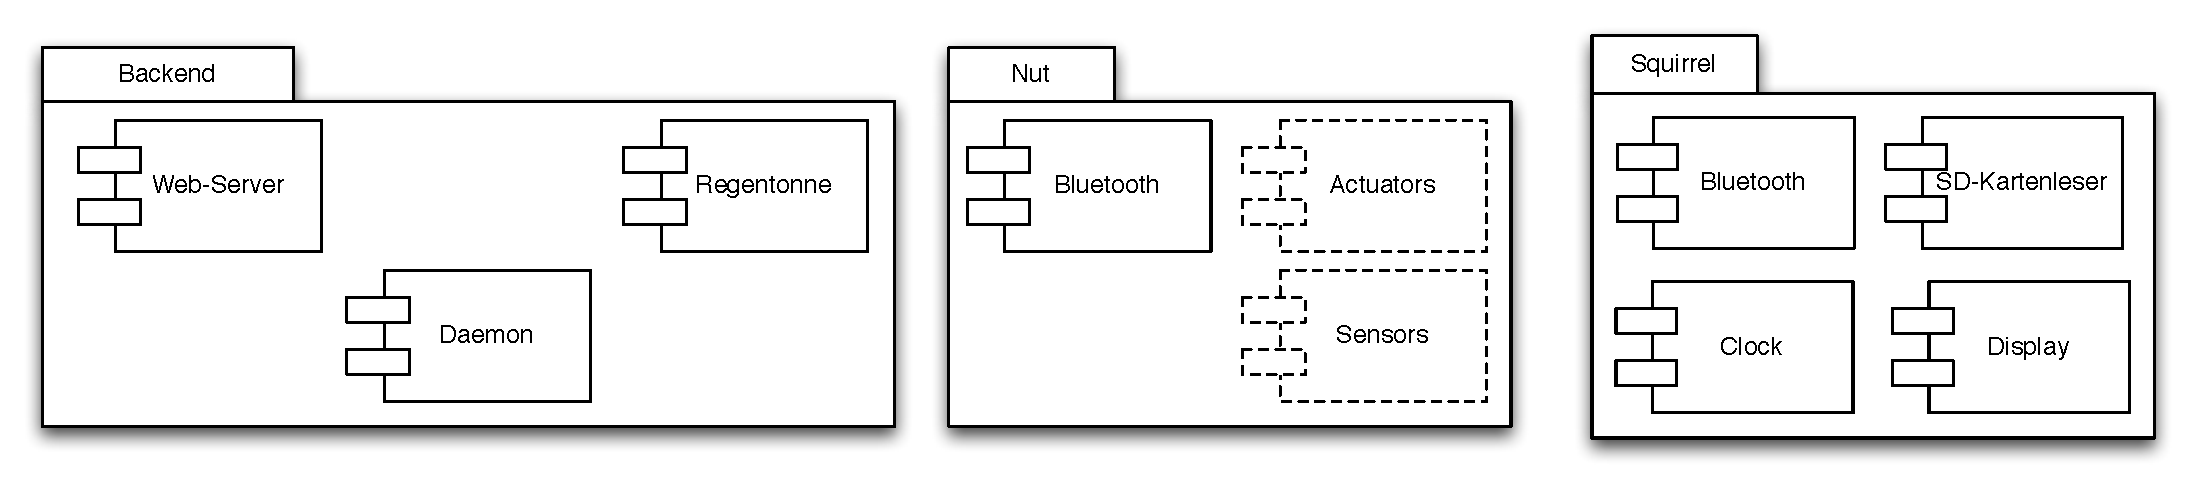
\includegraphics[height=4.2cm]{./Deployment.pdf}

	\subsection{Squirrel}
	\subsubsection{Prozessor}
	Die Squirrel verfügt über einen Atmel XMega128A1 Prozessor.\\
	Dieser hat eine Taktrate von 32 Mhz und 128KB Arbeitsspeicher.\\
	
	
%realtimeclock erwähnen und tasten
	\subsubsection{Bluetooth}
	\label{bluetooth}
Das Bluetooth-Modul ist über UART mit dem XMEGA-Prozessor verbunden. Im Bluetooth-Stack gibt es zwei Modi. \\
Zun einen den Command-Modus, welcher dazu dient Befehle direkt an das Bluetooh-Modul zu senden.\\
Desweiteren gibt es den Communication-Modus der dann die tatsächlichen Bluetooth-Befehle versendet.\\
Die empfangenen Daten werden in einer Fifo-Datenstruktur gespeichert.\\


\subsubsection{Display: SDL-Emulation}
Um die Funktionsfähigkeit des Display-Treibers auch ohne Hardwarezugriff testen zu können, wurde eine SDL-Emulation geschrieben.\\
Sie bietet die Möglichkeit in einem SDL-Fenster die Ausgabe ähnlich wie auf dem Display auszugeben.\\
Somit konnten alle GUI-Libary-Ausgaben bereits im voraus getestet werden und mehrere Programmierer in die Entwicklung von neuen GUI-Anwendungen einbezogen werden, ohne durch die Verfügbarkeit der Hardware eingeschränkt zu sein.\\
Um die SDL-Emulation zu Nutzen, muss bei der Compilation des Display-C-Dateien das define x86 gesetzt werden.\\

\subsubsection{SD-Kartenleser}
Um den Nutzer die Möglichkeit zu geben, Messendatenprotokolle direkt aus der Squirrel unter Umgehung des Backends zu erhalten.
Damit die Daten direkt in der Gewohnten Betriebsystemumgebung am PC des Anwenders auslesen zu können, ist es notwendig die Daten in einem weit verbreiteten Dateisystem abzulegen.\\
Hierbei fiel die Wahl auf das FAT16 System, da es gegenüber FAT32 eine einfachere Struktur besitzt und trotzdem Speicherkarten bis 2GB unterstützt. Somit allen Anforderungen gerecht werden.\\
Die Squirrel verfügt über die Fähigkeit Dateien zu
\begin{itemize}
\item öffnen
\item lesen
\item schreiben
\item löschen
\end{itemize}
Außerdem können Verzeichnisse angelegt, entfernt und durchsucht werden.\\


\begin{figure}[h]
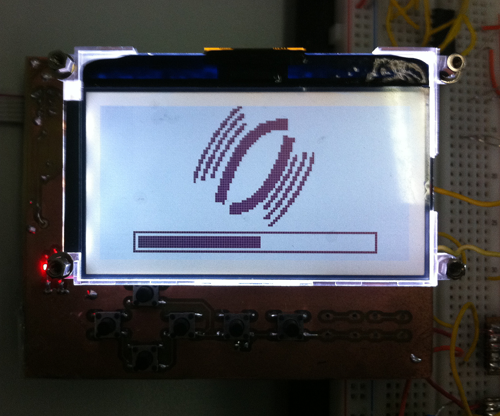
\includegraphics[height=5cm]{squirrel_shot1.png}
\label{fig:0}
\caption{Squirrel}
\end{figure}
\begin{figure}[h]
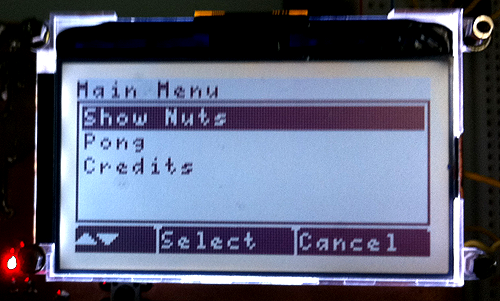
\includegraphics[height=5cm]{squirrel_shot2.png}
\label{fig:1}
\caption{Squirrel}
\end{figure}


\subsection{Nut}

Die hier aufgeführte Hardware stellt das Grundgerüst einer Nut da.
Zur Verbesserung der Kompatibilität ist das selbe Bluetooth-Modul gewählt worden. Diese Wahl wirkte sich durch verringerte Einarbeitungszeit positiv auf den Entwicklungsprozess aus.

\subsubsection{Prozessor}
Die Nut verfügt über einen Atmel Atmega8535 Prozessor.\\
Dieser hat eine Taktrate von 16 MHz und 8KB Arbeitsspeicher.\\


\subsubsection{Bluetooth}
Siehe Abschnitt~\ref{bluetooth}


\section{Wetterstation}
	\subsection{Funktionen}
	Die Wetterstation erfasst Luftdruck, Umgebungstemperatur, Helligkeit und Luftfeuchtigkeit. Desweiteren verfügt sie über zwei rote LED's, welche an und abgeschaltet werden können.
	\subsection{Hardware}
		\subsubsection{Drucksensor (BMP085)}
		Der Drucksensor ist durch $\text{I}^2$C angebunden und kann Drücke zwischen 300 hPa und 1100 hPa mit einer Genauigkeit von 16bit erfassen.
		\subsubsection{Temperatursensor (BMP085)}
		Der ist selben Chip wie der Drucksenor integriert und gibt in 0.1 Cº die Temperatur in einem 16 Bit-Wert aus.
		\subsubsection{Lichtstärke (Photoresistor)}
		Die Lichtstärke wird von einem Photoresitor gemessen und der AVR liest diesen analogen Wert durch einen Analog-Digital-Converter (ADC) ein. Es kann eine Helligkeit von 0,1 Lux bis 1000 Lux in einer Schrittweite von 10 Lux gemessen werden.
		\subsubsection{Feuchtigkeitssensor (HIH3001)}
		Der Feuchtigkeitssensor HIH3001 misst die relative Luftfeuchtigkeit in \% in ganz kleinen Schritten. 

		\begin{figure}[h]
		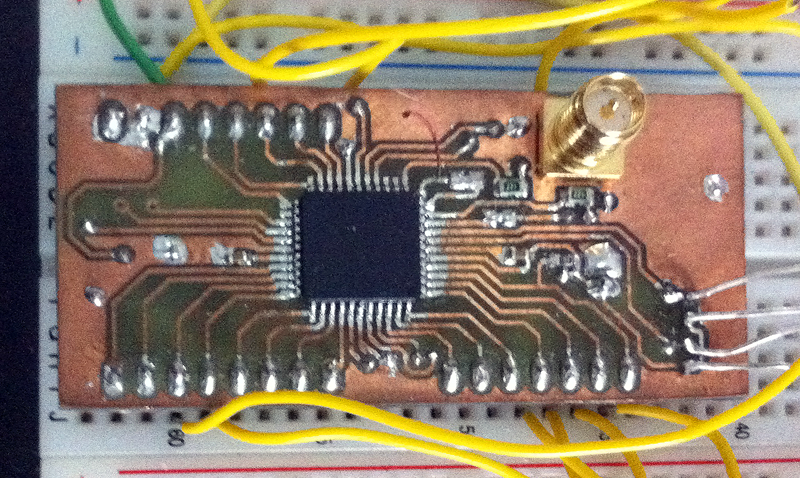
\includegraphics[height=5cm]{nut_shot1.png} 
		\label{fig:2}
		\caption{Nut}
		\end{figure}

		
\section{Backend}
Das Backend stellt eine Web-Oberfläche zur Verfügung über die es möglich ist Log-Daten aus der Squirrel grafisch aufbereitet darzustellen oder Aktor-Befehle an die angeschlossenen Geräte zu senden. Das Backend besteht aus einem in Java geschriebenen Daemon sowie einer in Perl geschriebenen Web-Oberfläche die via CGI über einen Webserver verfügbar gemacht wird.

\subsubsection{Daemon}
Der Daemon ist ein in Java geschriebenes Programm, welches mit Hilfe der Bluecove-Libary die Aktivitäten des Squirrels - und somit des gesamten Almond-Systems - überwacht.\\
Die anfallenden Log-Daten werden in einer SQLite-Datenbank gespeichert.\\
Außerdem überprüft es in der Datenbank, ob mit Hilfe des Web-Interfaces Aktoren gesteuert werden. Ist dies der Fall, werden die entsprechenden Kommandos direkt über Bluetooth mit dem Downlinkprotokoll - unter Umgehung des Squirrels - an die Nuts gesendet.\\

\subsubsection{Datenbank}
Als Datenbank wird auf MySQL Server zurückgegriffen. Auf dem Backend-System welches den Webserver zur Verfügung stellt wird ein MySQL vorrausgesetzt das auch zur Kommunikation zwischen der Web-Oberfläche und dem Java-Daemon dient. \\
Das launch-Script des Backends liest Zugangsdaten und Schema-Name aus der Konfigurationsdatei und legt die benötigten Tabellen an.

\subsubsection{Web-Server}
Das Backend nutzt als Benutzeroberfläche eine in Perl geschriebene Web-Anwendung, was Nutzung von mehreren Web-Fähigen Geräten aus einfach macht. Die Web-Oberfläche kann als Virtual-Host in einen vorhandenen Webserver (z.B. Apache oder lighttpd) integriert werden. Vorraussetzung ist eine perl Runtime, einige Perl-Module (siehe README.txt im Backend) sowie ein CGI fähiger Webserver. Ist ein lighttpd auf dem Server-System installiert der nicht genutzt wird, kann das launch-Script diesen mit einer bereits vorkonfigurierten Datei starten und das Web-Interface läuft ohne weitere Modifikationen.
Das launch-Script des Backends startet auch den Java-Daemon, der über die MySQL Datenbank dann mit der Oberfläche kommuniziert.
		
\section{Team}
Hier eine grafische Übersicht der Teammitglieder und deren Tätigkeitsbereiche:\\
\begin{multicols}{2}{
\begin{list}{ }
	\item    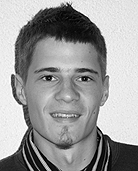
\includegraphics[height=1.5cm]{./face_Fanter.png}     \\      Stefan Profanter	
	\item    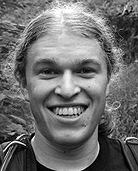
\includegraphics[height=1.5cm]{./face_Lotz.png}       \\      Linus Lotz 
	\item    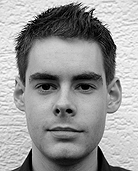
\includegraphics[height=1.5cm]{./face_Matthias.png}   \\      Matthias Schwab	
	\item    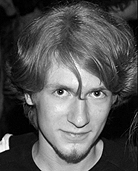
\includegraphics[height=1.5cm]{./face_Maxikay.png}    \\      Maximilian Karl
	\item    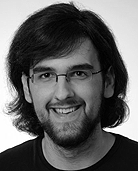
\includegraphics[height=1.5cm]{./face_Parsch.png}     \\      Thomas Parsch		
	\item 	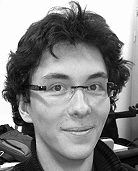
\includegraphics[height=1.5cm]{./face_Rupprecht.png}   \\      Christian Rupprecht
	\item    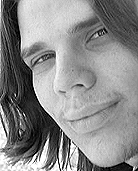
\includegraphics[height=1.5cm]{./face_Schnurrrr.png}  \\      Pascal Schnurr    
	\item    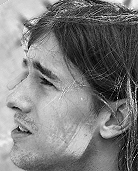
\includegraphics[height=1.5cm]{./face_Schon.png}      \\      Seán Labastille   
	\item    
\includegraphics[height=1.5cm]{./face_Sickert.png}    \\      Salomon Sickert
\end{list}
}
\end{multicols}


\section{Entwicklungeschichte}
\subsection{Display}
Zunächst wurde zum Entwickeln des Display-Treibers auf eine Test-Hardware zurückgegriffen, in der ebenfalls ein 13BB0-Display verbaut worden war.\\
Das ursprünglich in einem DVB-T Receiver eingesetzte Board verfügt jedoch nur nur über den schwächeren ATMEGA 8515, welcher über weniger Speicher verfügt.\\
Daher wurde zunächst ein Programm entwickelt, das nur wenig Platz verbraucht und trotzdem die notwendige Flexibilität bietet, beliebige Inhalte anzuzeigen.\\
Um Buchstaben komfortabel für dieses Programm codieren zu können, wurde ein Hilfsprogramm in Java erstellt, welches eine Grafische Oberfläche bietet zum Entwerfen der Buchstaben.\\
Im Laufe der Entwicklung stellte sich jedoch heraus, dass nicht nur eine Darstellung von Buchstaben an bestimmten fixen Plätzen auf dem Display benötigt wird, sondern eine noch flexiblere pixelweise Ansteuerung.\\
Da die endültige Hardware des Squirrels über mehr Speicher verfügt, war dies durch ein Neuschreiben vieler Teile des Display-Treibers möglich.\\
 Um das den weitgehen neuen Display Treiber mit verschiedenen Schriftarten versorgen zu können, wurde ein Perl-Skript geschrieben, welches die Standardfonts der GD-Libary konvertieren kann.\\



\subsection{Bluetooth}
Zunächst wurde ein eher monolithischer Bluetooth-Stack geschrieben, dies führte jedoch zu einem Komplexitätsproblem.\\
Folglich wurde ein neuer leichtgewichtigerer und übersichtlicher Stack entworfen.


\end{document}
